\chapter{Software}
\label{chap:software}
Die Software die im Rahmen dieser Arbeit entwickelt wurde, ist in C++ geschrieben. Als Entwicklungsumgebung wurde Eclipse mit den \ac{CDT} auf einem Linux\footnote{Ubuntu 12.04 LTS}  Betriebssystem verwendet.
\section{Simulation}
\label{sec:simulation}
Grundlage der Simulation ist das 3D Grafiktoolkit \ac{OCG}\footnote{\url{http://www.openscenegraph.org/}}. Damit l�sst sich eine 3D Szene in Form eines Graphen aufbauen und mit einem Viewer darstellen. Um den Ablauf kontrollieren zu k�nnen, l�sst sich die Render-Schleife manuell aufrufen um jeden Frame einzeln berechnen zu lassen. Dies wurde als Simulationsschritt gew�hlt in dem alle n�tigen Berechnungen durchgef�hrt werden k�nnen. Da die Geschwindigkeit mit der die Simulation im manuellen Modus abl�uft nicht begrenzt wird, wurde eine Mindestbearbeitungszeit integriert. Denn die Geschwindigkeiten von Objekten in der Simulation, wie dem Roboter, werden durch eine zur�ckgelegte Strecke pro Simulationsschritt festgelegt. Bei sehr schneller Hardware ergab dies eine zu hohe Bewegungsrate um den Roboter noch manuell steuern zu k�nnen. F�r automatisierte Simulationsl�ufe mit festgelegten Fahrprofilen k�nnte man diese Begrenzung wieder l�sen um Zeit zu sparen.

\subsection{Die Szene}
\label{subsec:dieSzene}
\begin{description} 
\item[Die Grundfl�che] der B�hne misst 12 x 12 m. Sie wird als einfach wei�e Fl�che in der Szene dargestellt. Da die Bildverarbeitung nur auf den Oberen Teil des Bildes beschr�nkt ist, spielen Farbe und Helligkeit keine Rolle bei der Erkennung des Musters im Bild.
\end{description}
 
\begin{figure}[h]
    \centering
    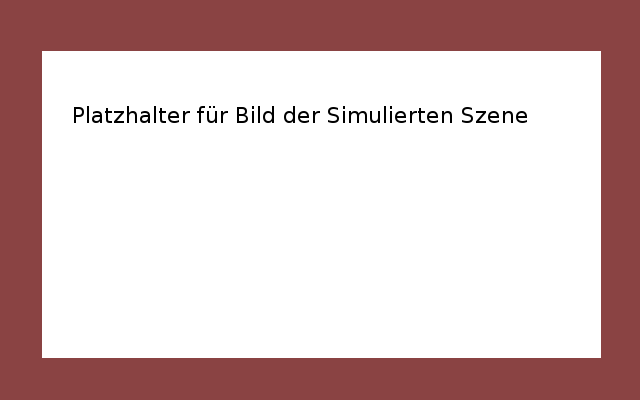
\includegraphics[width=\textwidth]{chapter2.2/bildderszene.png}
    \caption[Bild Simulierte Szene]{Bild Simulierte Szene}
    \label{fig:bildderszene}
\end{figure}

\begin{description}
\item[Die Lichtw�nde] sind zu drei Seiten der Grundfl�che aufgestellt. Sie messen 3m in der H�he und 8m  in der L�nge. Wie bereits in #### beschrieben soll das Muster in der obersten Zeile der Lichtw�nde dargestellt werden. Hierzu k�nnen verschiedene Texturen geladen werden die das Bitmuster enthalten. In den Lichtw�nden auf der B�hne 
\end{description}

\section{Lokalisation}
\label{sec:lokalisation}

